\section{Implementation}

\subsection{Parameters}
A schematic showing the trombone geometry is shown in Figure \ref{fig:tromboneSchematic} and the lengths and radii used in Table \ref{tab:geometry}.

Other parameters used in the simulation can be found in Table \ref{tab:parameters}.


\begin{table}[t]
    \small
    \begin{center}
    \begin{tabular}{|l|c|c|}
        \hline
        Part of tube & Length (cm) & Radius (cm)\\\hline
        Inner slide (1) & 70.8 & 0.69\\
        Outer slide (extended) (2) & 53 & 0.72 
        \\
        Slide crook (3)& 17.7 & 0.74\\
        Outer slide (extended) (4) & 53 & 0.72 
        \\
        Inner slide (5) & 71.1 & 0.69\\
        Gooseneck (6) & 24.1 & 0.71\\
        Tuning slide (7) & 25.4 & 0.75, 1.07\\
        Bell flare (8) & 56.7 \SWcomment[$\leftarrow$check]& 1, 10.8\\\hline
    \end{tabular}
    \caption{Geometry of a measured trombone taken from \cite{Smyth2011}. Numbers correspond to Figure \ref{fig:tromboneSchematic}.\label{tab:geometry}}
    \end{center}
\end{table}

\begin{figure}[ht]
    \centering
    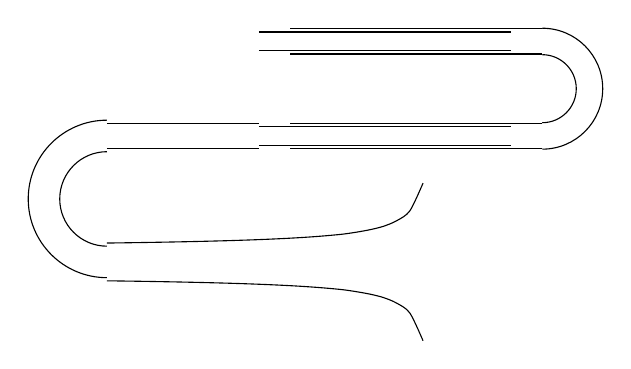
\begin{tikzpicture}[scale = 8]

    \def\hornOffset{0.02};
    \def\stepSize{0.005}

    % tuning slide params
    \def\tuningSlideDim{0.1};
    \pgfmathsetmacro{\tuningSlideRad}{\stepSize + \hornOffset};

    % gooseneck params
    \def\gooseNeckLength{0.241};
    \pgfmathsetmacro{\gooseNeckRad}{\tuningSlideRad - \stepSize};

    % inner slide params
    \def\innerLength{0.4};
    \pgfmathsetmacro{\innerRad}{\gooseNeckRad - \stepSize};

    % outer slide params
    \def\outerLength{\innerLength};
    \pgfmathsetmacro{\outerRad}{\gooseNeckRad};
    \pgfmathsetmacro{\extension}{0.05};

    \def\endOfSlideDim{0.075};
    \pgfmathsetmacro{\endOfSlideRad}{\outerRad * 1.05};

    %% draw horn
    % \filldraw[black] (0, 0) circle (0.1pt) node[anchor=west](origin){\tiny(0, 0)}; 

    \draw[domain=0:0.502, smooth, variable=\x, black] plot ({\x}, {\hornOffset + 0.0063 * ((0.502-\x) + 0.0174)^(-0.7)});
    
    \draw[domain=0:0.502, smooth, variable=\x, black] plot ({\x}, {-\hornOffset-0.0063 * ((0.502-\x) + 0.0174)^(-0.7)});
    
    % draw tuningSlide
    \pgfmathsetmacro{\innerTuningSlideDim}{(\tuningSlideDim - \tuningSlideRad)}
    \pgfmathsetmacro{\outerTuningSlideDim}{(\tuningSlideDim + \tuningSlideRad)}

    % \draw (0, 0) arc(270:90:\tuningSlideDim cm and \tuningSlideDim cm);

    % \filldraw[black] (0, 2*\tuningSlideDim) circle (0.1pt) node[anchor=west](origin){\tiny (0, 0.2)}; 

    \draw (0, \tuningSlideRad) arc(270:90:\innerTuningSlideDim cm and \innerTuningSlideDim cm);

    \draw (0, -\tuningSlideRad) arc(270:90:\outerTuningSlideDim cm and \outerTuningSlideDim cm);

    % draw gooseneck
    \draw (0, 2*\tuningSlideDim + \gooseNeckRad) -- (\gooseNeckLength, 2*\tuningSlideDim + \gooseNeckRad);

    \draw (0, 2*\tuningSlideDim - \gooseNeckRad) -- (\gooseNeckLength, 2*\tuningSlideDim - \gooseNeckRad);

    % draw inner slide
    \draw (\gooseNeckLength, 2*\tuningSlideDim + \innerRad) -- (\gooseNeckLength+\innerLength, 2*\tuningSlideDim + \innerRad);

    \draw (\gooseNeckLength, 2*\tuningSlideDim - \innerRad) -- (\gooseNeckLength+\innerLength, 2*\tuningSlideDim - \innerRad);

    % draw outer slide
    \pgfmathsetmacro{\outerSlideStart}{\gooseNeckLength + \extension};

    \draw (\outerSlideStart, 2*\tuningSlideDim + \outerRad) -- (\outerSlideStart+\outerLength, 2*\tuningSlideDim + \outerRad);

    \draw (\outerSlideStart, 2*\tuningSlideDim - \outerRad) -- (\outerSlideStart+\outerLength, 2*\tuningSlideDim - \outerRad);

    % draw end of slide
    \pgfmathsetmacro{\innerEndOfSlideDim}{(\endOfSlideDim - \endOfSlideRad)};
    \pgfmathsetmacro{\outerEndOfSlideDim}{(\endOfSlideDim + \endOfSlideRad)};

    \pgfmathsetmacro{\startEndOfSlide}{\outerSlideStart + \outerLength};

    \draw (\startEndOfSlide, 2*\tuningSlideDim+\endOfSlideRad) arc(-90:90:\innerEndOfSlideDim cm and \innerEndOfSlideDim cm);

    \draw (\startEndOfSlide, 2*\tuningSlideDim-\endOfSlideRad) arc(-90:90:\outerEndOfSlideDim cm and \outerEndOfSlideDim cm);

    % draw second outer slide

    \draw (\outerSlideStart, 2*\tuningSlideDim + 2 * \endOfSlideDim + \outerRad) -- (\outerSlideStart+\outerLength, 2*\tuningSlideDim + 2 * \endOfSlideDim + \outerRad);

    \draw (\outerSlideStart, 2*\tuningSlideDim + 2 * \endOfSlideDim - \outerRad) -- (\outerSlideStart+\outerLength, 2*\tuningSlideDim + 2 * \endOfSlideDim - \outerRad);

    % draw inner slide
    \draw (\gooseNeckLength, 2*\tuningSlideDim+ 2 * \endOfSlideDim + \innerRad) -- (\gooseNeckLength+\innerLength, 2*\tuningSlideDim+ 2 * \endOfSlideDim + \innerRad);

    \draw (\gooseNeckLength, 2*\tuningSlideDim + 2 * \endOfSlideDim - \innerRad) -- (\gooseNeckLength+\innerLength, 2*\tuningSlideDim + 2 * \endOfSlideDim - \innerRad);

% \begin{scope}[very thick,decoration={
%     markings,
%     mark=at position 0.5 with {\arrow{>}}}
%     ] 
%     \draw[postaction={decorate}] (-4,0)--(4,0);
% \end{scope}
    
    \end{tikzpicture}
    \caption{Lipsystem with the equilibrium at 0 and the distance from the lower lip $H_0$.}
    \label{fig:lipSystem}
\end{figure}

\begin{table}[t]
    \small
    \begin{center}
    \begin{tabular}{|l|c|c|}
        \hline
        Name & Symbol (unit) & Value\\ \hline
        \multicolumn{3}{|l|}{\bf Tube}\\ \hline
        Length & $L$ (m) & $2.685\leq L \leq 3.718$$^\star$\\
        Air density &$\rho_0$ (kg/m$^3$) & 1.1769** 
        \\
        Wave speed & $c$ (m/s) & 347.23**\\
        Geometry & $S$ (m$^2$) & See Table \ref{tab:geometry}. \\\hline
        \multicolumn{3}{|l|}{\bf Lip reed}\\ \hline
        Mass & $M_\text{r}$ (kg) & $5.37\cdot10^{-5}$*\\
        Frequency & $\omega_0$ (rad/s) & $\SWcomment[??] \leq \omega_0 \leq \SWcomment[??]$\\
        Mouth pressure & $P_\text{m}$ (Pa) & $0 \leq P_\text{m} \leq 6000\SWcomment[??]$\\
        Damping & $\sigma_\text{r}$ (s$^{-1}$) & $5$*\\
        Eff. surface area & $S_\text{r}$ (m$^{2}$) & $1.46\cdot 10^{-5}$*\\
        Width & $w_\text{r}$ (m) & $0.01$* \\
        Equilibrium sep. & $H_0$ (m) &  $2.9 \cdot 10^{-4}$* \\
        Coll. stiffness& $K_\text{c}$ (N/m) & $10^4$\\
        Nonlin. coll. coeff.& $\alpha_\text{c}$ (-)  &3\\\hline

    \end{tabular}
    \caption{List of parameter values used for the simulation. 
    Taken from $^\star$\cite{Smyth2011}, *\cite{Harrison2018} or **\cite{Benade1968} with temperature $T=26.85^\circ C$. \label{tab:parameters}}
    \end{center}
\end{table}

\subsection{Limit on speed of change}
u
\subsection{Order of Calculation}